\documentclass[letterpaper,12pt,oneside]{article}\usepackage[]{graphicx}\usepackage[]{color}
%% maxwidth is the original width if it is less than linewidth
%% otherwise use linewidth (to make sure the graphics do not exceed the margin)
\makeatletter
\def\maxwidth{ %
  \ifdim\Gin@nat@width>\linewidth
    \linewidth
  \else
    \Gin@nat@width
  \fi
}
\makeatother

\definecolor{fgcolor}{rgb}{0.345, 0.345, 0.345}
\newcommand{\hlnum}[1]{\textcolor[rgb]{0.686,0.059,0.569}{#1}}%
\newcommand{\hlstr}[1]{\textcolor[rgb]{0.192,0.494,0.8}{#1}}%
\newcommand{\hlcom}[1]{\textcolor[rgb]{0.678,0.584,0.686}{\textit{#1}}}%
\newcommand{\hlopt}[1]{\textcolor[rgb]{0,0,0}{#1}}%
\newcommand{\hlstd}[1]{\textcolor[rgb]{0.345,0.345,0.345}{#1}}%
\newcommand{\hlkwa}[1]{\textcolor[rgb]{0.161,0.373,0.58}{\textbf{#1}}}%
\newcommand{\hlkwb}[1]{\textcolor[rgb]{0.69,0.353,0.396}{#1}}%
\newcommand{\hlkwc}[1]{\textcolor[rgb]{0.333,0.667,0.333}{#1}}%
\newcommand{\hlkwd}[1]{\textcolor[rgb]{0.737,0.353,0.396}{\textbf{#1}}}%

\usepackage{framed}
\makeatletter
\newenvironment{kframe}{%
 \def\at@end@of@kframe{}%
 \ifinner\ifhmode%
  \def\at@end@of@kframe{\end{minipage}}%
  \begin{minipage}{\columnwidth}%
 \fi\fi%
 \def\FrameCommand##1{\hskip\@totalleftmargin \hskip-\fboxsep
 \colorbox{shadecolor}{##1}\hskip-\fboxsep
     % There is no \\@totalrightmargin, so:
     \hskip-\linewidth \hskip-\@totalleftmargin \hskip\columnwidth}%
 \MakeFramed {\advance\hsize-\width
   \@totalleftmargin\z@ \linewidth\hsize
   \@setminipage}}%
 {\par\unskip\endMakeFramed%
 \at@end@of@kframe}
\makeatother

\definecolor{shadecolor}{rgb}{.97, .97, .97}
\definecolor{messagecolor}{rgb}{0, 0, 0}
\definecolor{warningcolor}{rgb}{1, 0, 1}
\definecolor{errorcolor}{rgb}{1, 0, 0}
\newenvironment{knitrout}{}{} % an empty environment to be redefined in TeX

\usepackage{alltt}
\usepackage[paperwidth=8.5in,paperheight=11in,top=1in,bottom=1in,left=1in,right=1in]{geometry}
\usepackage{setspace}
\usepackage[colorlinks=true,allcolors=Blue]{hyperref}
\usepackage[usenames,dvipsnames]{xcolor}
\usepackage{indentfirst}
\usepackage{titlesec}
\usepackage{multirow}
\usepackage{booktabs}
\usepackage{graphicx}
\usepackage{verbatim}
\usepackage{rotating}
\usepackage{tabularx}
\usepackage{outlines}
\usepackage{lineno}
\usepackage{array}
\usepackage{times}
\usepackage{cleveref}
\usepackage{acronym}
\usepackage[position=t]{subfig}
\usepackage{paralist}
\usepackage[noae]{Sweave}
\usepackage{natbib}
\usepackage{array}
\usepackage{pdflscape}
\usepackage{bm}
% \usepackage{showlabels}
\bibpunct{(}{)}{,}{a}{}{,}

% page margins and section title formatting
\linespread{2}
\setlength{\footskip}{0.5in}
\titleformat*{\section}{\Large\bf\em}
\titleformat*{\subsection}{\singlespace\large\bf}
\titleformat*{\subsubsection}{\singlespace\normalsize\bf\em}
\titlespacing{\section}{0in}{0in}{0in}
\titlespacing{\subsection}{0in}{0in}{0in}
\titlespacing{\subsubsection}{0in}{0in}{0in}

% cleveref options
\crefname{table}{Table}{Tables}
\crefname{figure}{Fig.}{Figs.}
\renewcommand{\figurename}{Fig.}

% aliased citations
\defcitealias{HagyIR}{Hagy, In review}

%acronyms
\acrodef{DEM}{Digital Elevation Model}
\acrodef{EPA}{Environmental Protection Agency}
\acrodef{doc}[DoC]{depth of colonization}
\acrodef{GIS}{Geographic Information System}
\acrodef{NOAA}{National Oceanic and Atmospheric Administration}

%knitr options


% example of buffer points for depth of col


% example of estimating seagrass depth of colonization


\IfFileExists{upquote.sty}{\usepackage{upquote}}{}
\begin{document}

\raggedbottom
\linenumbers
\raggedright
\urlstyle{same}
\setlength{\parindent}{0.5in}
\renewcommand\refname{References \vspace{12pt}}

\begin{singlespace}
\title{{\bf {\Large Improving spatial resolution in estimates of seagrass depth of colonization}}}
\author{
  {\bf {\normalsize Marcus W. Beck$^1$, James D. Hagy III$^2$}}
  \\\\{\textit {\normalsize $^1$ORISE Research Participation Program}}
  \\{\textit {\normalsize USEPA National Health and Environmental Effects Research Laboratory}}
  \\{\textit {\normalsize Gulf Ecology Division, 1 Sabine Island Drive, Gulf Breeze, FL 32561}}
	\\{\textit {\normalsize Phone: 850-934-2480, Fax: 850-934-2401, Email: \href{mailto:beck.marcus@epa.gov}{beck.marcus@epa.gov}}}
  \\\\{\textit {\normalsize $^2$USEPA National Health and Environmental Effects Research Laboratory}}
	\\{\textit {\normalsize Gulf Ecology Division, 1 Sabine Island Drive, Gulf Breeze, FL 32561}}
	\\{\textit {\normalsize Phone: 850-934-2455, Fax: 850-934-2401, Email: \href{mailto:hagy.jim@epa.gov}{hagy.jim@epa.gov}}}
	}
\date{}
\maketitle
\end{singlespace}
\clearpage

\section{Introduction}

\section{Methods}

Development of a spatially-referenced approach to estimate seagrass \ac{doc} relied extensively on data and partially on methods described in \citetalias{HagyIR}.  The following is a summary of locations and data sources, methods in \citetalias{HagyIR}, methods and rationale developed to incorporate spatial information in seagrass \ac{doc}, and evaluation of the approach including relationships with water clarity.   

\subsection{Locations and data sources}

Four unique locations were chosen for the analysis: Choctowatchee Bay (Panhandle), Big Bend region (northeast Gulf of Mexico), Tampa Bay (central Gulf Coast of Florida), and Indian River Lagoon (east coast) ().  These locations were chosen to represent the different geographic regions in the state, in addition to data availability and observed gradients in water clarity that likely contributed to hetereogeneity in seagrass growth patterns.  For example, the Big Bend region was chosen to an outflow of the Steinhatchee River where higher concentrations of dissolved organic matter are observed.  Seagrasses near the outflow were observed to grow at shallower depths as compared to locations far from the river source.  Coastal regions and estuaries in Florida are divided into individual spatial units based on a segmentation scheme developed by US \ac{EPA} for the development of numeric nutrient criteria.  One segment from each geographic location was used for the analysis to evaluate estimates of seagrass \ac{doc}.  The segments included numbers 0303 (Choctowatchee Bay), 0820 (Big Bend region), 0902 (Tampa Bay), and 1502 (Indian River Lagoon), where the first two digits indicate the estuary and the last two digits indicate the segment within the estuary. 

Data used to estimate seagrass \ac{doc} included a suite of publically available \ac{GIS} products.  At the most generic level, spatially-referenced information describing seagrass aerial coverage combined with co-located bathymetric depth information were used to estimate \ac{doc}.  These data products are available in coastal regions of Florida through the US Geological Survey, Florida Department of Environmental Protection, and watershed management districts.  Data are generally more available in larger estuaries that are of specific management concern, e.g., Tampa Bay, Indian River Lagoon.  For example, seagrass coverage data are available from 1950 (Tampa Bay) to present day (multiple estuaries), with more recent products available at annual or  biennial intervals.  Seagrass coverage maps are less frequent in areas with lower population densities (e.g., Big Bend region) or where seagrass is naturally absent (northeast Florida).  Seagrass maps were produced using photo-interpretations of aerial images to categorize coverage as absent, discontinuous (patchy), or continuous.  For this analysis, we considered seagrass coverage as being only present (continuous and patchy) or absent since the former did not represent unequivocal categories between regions. 

Seagrass coverage maps were combined with bathymetric depth layers to characterize location and depth of growth in each location.  Bathymetric depth layers for each location were obtained from the National Oceanic and Atmospheric Administration's (\acsu{NOAA}) National Geophysical Data Center as either \acp{DEM} or raw sounding data from hydroacoustic surveys.  Tampa Bay data provided by the Tampa Bay National Estuary Program are described in \citet{Tyler07}. Bathymetic data for the Indian River Lagoon were obtained from the St. John's Water Management District \citep{CPE97}.  \ac{NOAA} products were referenced to mean lower low water, whereas Tampa Bay data were referenced to the North American Vertical Datum of 1988 and the Indian River Lagoon data were referenced to mean sea level.  Depth layers were combined with seagrass coverage layers using standard union techniques of raster and vector layers in ArcMap 10.1 \citep{ESRI12}.  To reduce computation time, depth layers were first masked using a 1 km buffer of the seagrass coverage layer.  The final layer used for analysis was a point layer with attributes describing location (latitude, longitude, segment), depth (m), and seagrass (present, absent).  Additional details describing the data are available in \citet{HagyIR}.    

\subsection{Segment-based estimates of seagrass depth of colonization}

Methods described in \citet{HagyIR} estimate seagrass \ac{doc} for individual coastal segments.  Specifically, the combined seagrass depth data described above are used to estimate maximum ($Z_{cMax}$) and median ($Z_{c50\%}$) seagrass \ac{doc}, where the maximum depth is defined as the deepest depth at which a ``significant'' coverage of seagrasses occured in a segment and the median depht is defined as the median depth occurring at the deep water edge. The seagrass depth points are grouped into bins and the proportion of points within each depth bin that contain seagrass are quantified.  Both seagrass \ac{doc} estimates are obtained from the plot of proportion of points occupied at each depth bin.  In general, the plot is characterized by a decreasing trend such that the proportion of occupied points by depth bin decreases and eventually flattens with increasing depth.  A regression is fit on this descending portion of the curve such that the intercept point on the x-axis is considered the maximum depth of colonization.  The median portion of this curve is considered the median depth of the deepwater edge of seagrass.   

Considerable spatial heterogeneity in the observed seagrass growth patterns suggests that a segment-wide estimate of seagrass \ac{doc} may be inappropriate, particularly for the chosen examples in the current analysis. \Cref{fig:wbid_doc} illustrates spatial variation in seagrass distribution on a latitudinal gradient in Old Tampa Bay, Florida.  Using methods in \citet{HagyIR}, the estimate for median seagrass \ac{doc} for the segment is an over- and under-estimate for northern and southern portions, respectively.  \Cref{fig:wbid_doc2} provides a similar example for the a segment in the Big Bend region of Florida.  Again, seagrass depth of colonization is over- and under-estimated for different areas of the segment.  In particular, \ac{doc} is greatly over-estimated at the outflow of the Steinhatchee where high concentrations of dissolved organic matter naturally limit seagrass growth.  These examples suggest that estimates of \ac{doc} are needed at finer spatial scales to provide a more robust determination of restoration targets and nutrient criteria.

\subsection{Estimating seagrass depth of colonization using spatial information}

The approach used to estimate seagrass \ac{doc} with spatial information has a similar theoretical foundation as the original, although several key differences should be noted.  The first difference is that the maximum \ac{doc} is estimated from a logistic growth curve fit through the data, as compared to a simple linear regression in the previous example.  The second and more important difference is that the estimates are specific to locations using a grid-based approach.  The implications and methods for using these differences are described below using an example from the Big Bend region of Florida.  Finally, a third measure describing the depth at which seagrass were most commonly located, as compared to maximum depth of growth, was defined using these methods.                                    

The spatially-referenced approach for estimating \ac{doc} begins by creating a grid of evenly-spaced sample points within the segment.  The same process for estimating \ac{doc} is used for each point.  Alternatively, a single location of interest can be chosen rather than a grid-based sampling design.  Seagrass depth data that occur within a set radius from the sampling point are selected (\cref{fig:buff_ex}).  An estimate of seagrass \ac{doc} is obtained using the selected seagrass depth points and assigned as a spatially-referenced value to each sampling point in the grid.  The seagrass \ac{doc} estimate for each sample point is quantified from the proportion of bathymetric soundings that contain seagrass at each depth bin in the data (\cref{fig:est_ex1}).  A buffer around a sample point that is sufficient to quantify depth of colonization typically has a plot similar to \cref{fig:est_ex1} such that the proportion of points that are occupied by seagrass decreases continuously with increasing depth.  

A decreasing logistic growth curve was then fit to the points to create a monotonic and asymptotic function to estimate depth of colonization.  This curve is fit using non-linear regression to characterize the reduction in points occupied by seagrass as a function of depth.  The logistic growth curve is fit using standard residual sums-of-squares and user-supplied starting parameters that are an approximate estimate of the curve characteristics.  The model has the following form:
\begin{equation}
 Proportion = \frac{\alpha}{1 + \mathrm{e}^{{\left(\beta - Depth\right)/\gamma}}}
\end{equation}
where the proportion of points occupied by seagrass at each depth is defined by a logistic curve with an asymptote $\alpha$, a midpoint inflection $\beta$, and a scale parameter $\gamma$.  Starting values $\alpha$, $\beta$, and $\gamma$ are estimated empirically from the observed data.  

Finally, a simple linear curve is fit through the inflection point ($\beta$) of the logistic curve to estimate depth of colonization (\cref{fig:est_ex3}).  The inflection point is the depth at which seagrass are decreasing at a maximum rate and is used as the slope of the linear curve.  Three measures are obtained from the linear curve. The maximum depth of seagrass colonization, $DOC_{max}$, is the x-axis intercept of the linear curve.  The depth of maximum seagrass occupany, $SG_{max}$ is the location where the linear curve intercepts the asymptote of the logistic growth curve.  The median depth of seagrass colonization, $DOC_{med}$, is the depth halfway between $SG_{max}$ and $DOC_{max}$.  $DOC_{med}$ was typically but not always the inflection point of the logistic growth curve.    

Estimates for each of the three \ac{doc} measures are obtained only if specific criteria are met.  These criteria were implemented to provide a safety measure that ensures a sufficient amount and appropriate quality of data are used in the calculations.  First, estimates can only be provided if a sufficient number of seagrass depth points are present within the radius of the sample point to estimate a logistic growth curve.  This criteria applies to the sample size as well as the number of points with seagrass in the sample.  That is, the curve cannot be estimated for small samples or if an insufficient number of points contain seagrass regardless of sample size.  Second, estimates are only provided if an inflection point is present on the logistic curve within the range of the depth data.  This criteria may apply under two scenarios where the curve is estimated but a trend is not adequately described by the observed data.  That is, a curve may be estimated that describes only the initial decrease in points occupied as a function of depth but the observed points do not occur at depths deeper than the predicted inflection point.  The opposite scenario may occur where a curve is estimated but only the deeper locations beyond the inflection point are present in the sample.  Finally, the estimate for $SG_{max}$ is set to zero if the linear curve through the inflection point intercepts the asympote at x-axis values less than zero.  The estimate for $DOC_{med}$ is also shifted to halfways between $SG_{max}$ and $DOC_{max}$.  All estimates were obtained using ...........

\subsection{Sensitivity analysis and comparison with segment-based approach}

\subsection{Developing a spatially coherent relationship of water clarity with depth of colonization}

\section{Results}

\section{Discussion}

% qualitative and quantitative advantages of the approach

%%%%%%
% refs
\clearpage
\begin{singlespace}
\bibliographystyle{apalike_mine}
\bibliography{ref_sgdepth}
\end{singlespace}
\clearpage

%%%%%%
% figures

% example of depth of col ests for wbid - Old Tampa Bay
\begin{figure}
\centerline{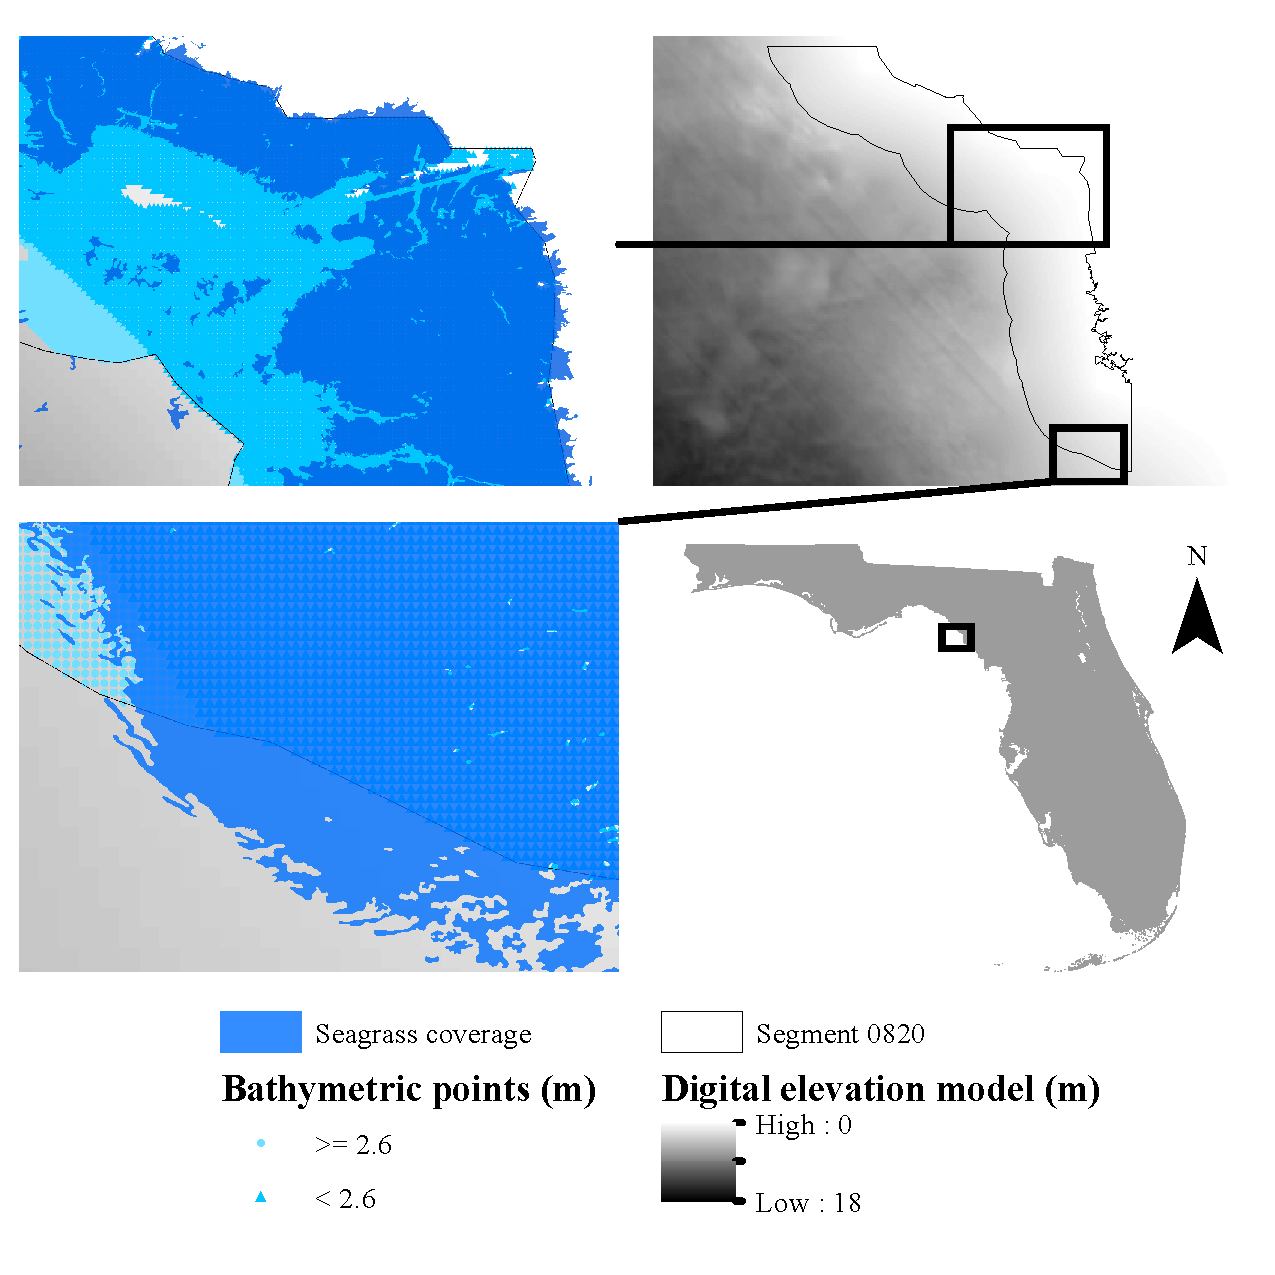
\includegraphics[width = \textwidth]{figs/wbid_doc.pdf}}
\caption{Example of over- and under-estimates for seagrass depth of colonization in Old Tampa Bay, Florida.  The top-left figure indicates over-estimation and the bottom-left indicates under-estimation.  Bathymetric points are color-coded by the median depth of colonization estimate for all seagrass (patchy and continuous) in the segment.}
\label{fig:wbid_doc}
\end{figure}

% example of depth of col ests for wbid - big bend 820
\begin{figure}
\centerline{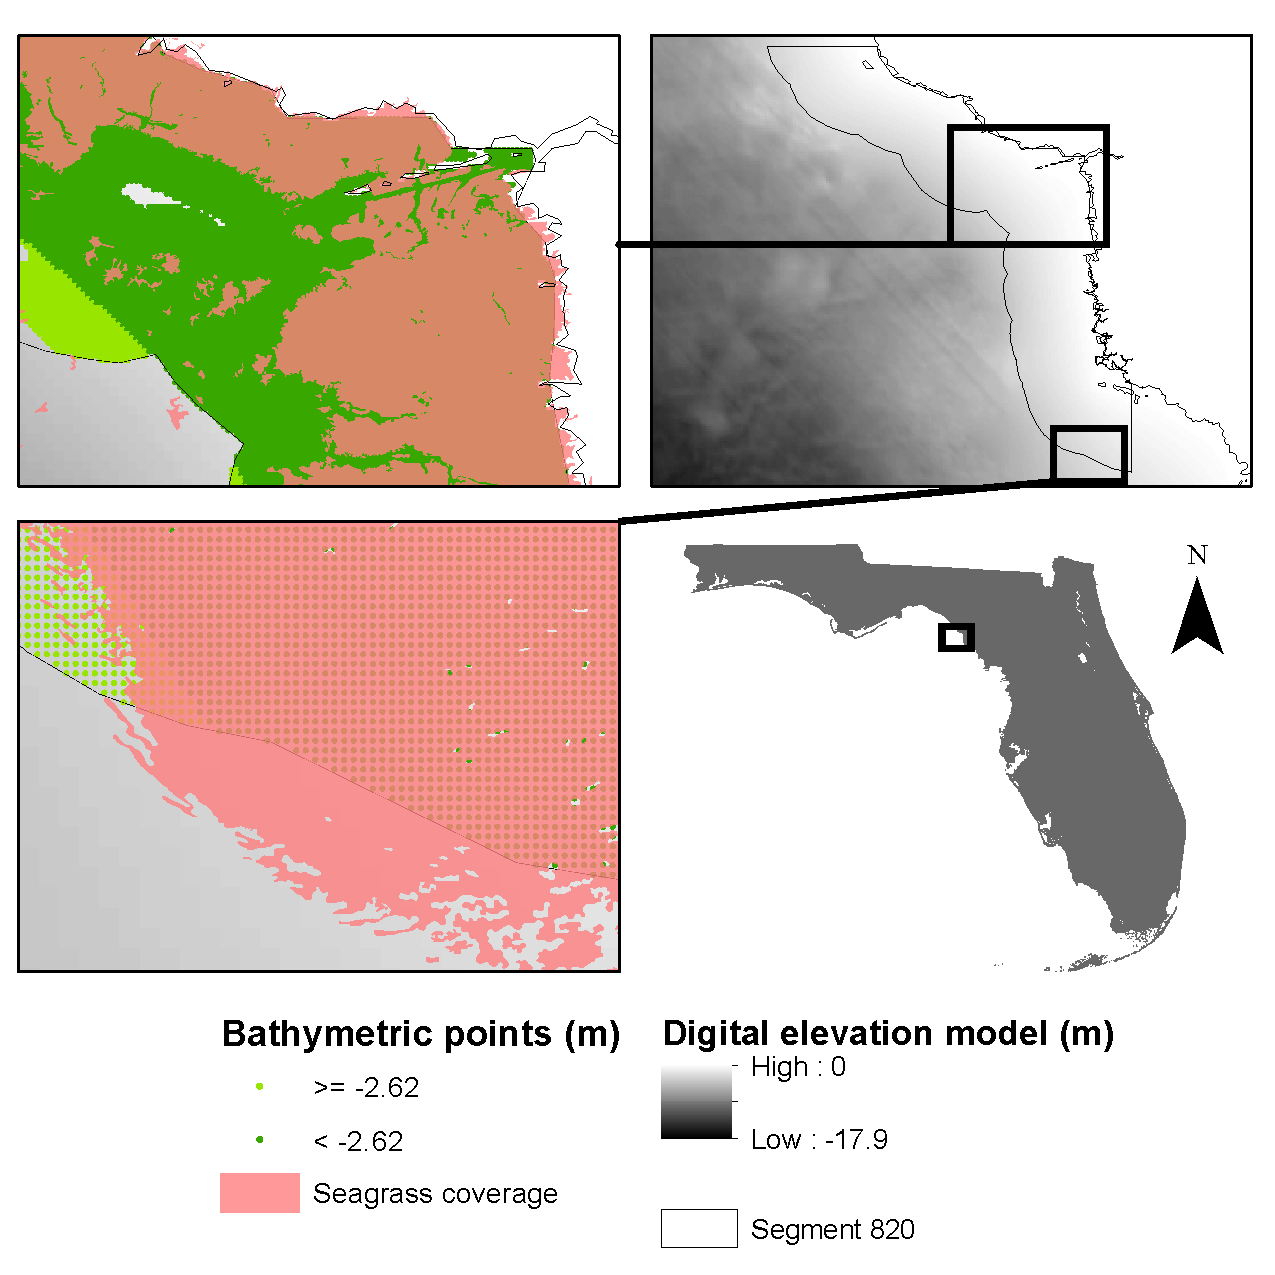
\includegraphics[width = \textwidth]{figs/wbid_doc2.pdf}}
\caption{Example of over- and under-estimates for seagrass depth of colonization for a segment in the Big Bend region, Florida.  The top-left figure indicates over-estimation and the bottom-left indicates under-estimation.  Bathymetric points are color-coded by the median depth of colonization estimate for continuous seagrass in the segment.}
\label{fig:wbid_doc2}
\end{figure}

% example of depth of col ests for wbid - big bend 820
\begin{figure}
\centerline{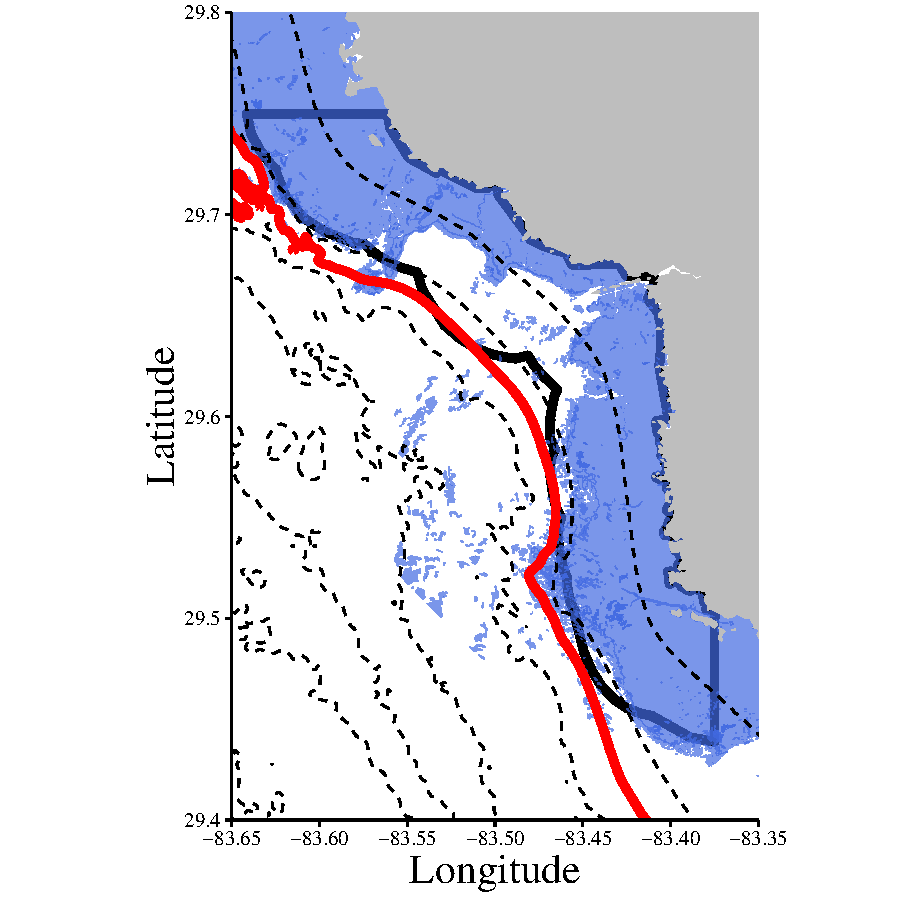
\includegraphics[width = 0.6\textwidth]{figs/buff_ex.pdf}}
\caption{Sample grid used to estimate spatially-referenced depth of colonization.  The selected bathymetric/seagrass points that were within a radius of 0.05 decimal degrees from the test point were selected for the estimate.  Estimates can be obtained for each sample grid point and an arbitrary radius.}
\label{fig:buff_ex}
\end{figure}

% example of depth of col ests for wbid - big bend 820
\begin{figure}
\centering
\subfloat[][Proportion of points with seagrass by depth]{
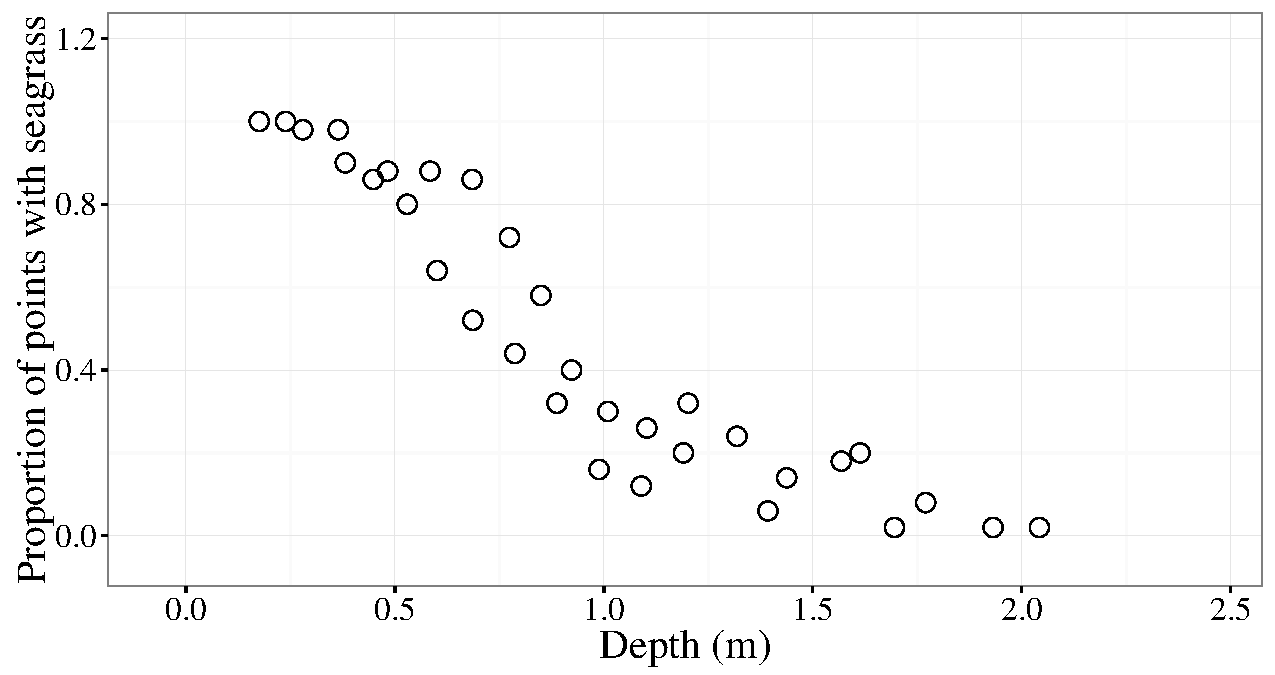
\includegraphics[page=1,width=0.5\textwidth]{figs/est_ex.pdf}
\label{fig:est_ex1}
}

\subfloat[][Logistic growth curve fit through points]{
\includegraphics[page=2,width=0.5\textwidth]{figs/est_ex.pdf}
\label{fig:est_ex2}
}

\subfloat[][Depth estimates]{
\includegraphics[page=3,width=0.5\textwidth]{figs/est_ex.pdf}
\label{fig:est_ex3}
}
\caption{Methods for estimating seagrass depth of colonization. \Cref{fig:est_ex1} is the proportion of points with seagrass by depth using depth points within the buffer of the test point in \cref{fig:buff_ex}.  \Cref{fig:est_ex2} adds a decreasing logistic growth curve fit through the points.  \Cref{fig:est_ex3} shows three depth estimates based on a linear curve fit through the inflection point of logistic growth curve.}
\label{fig:est_ex}
\end{figure}

\end{document}
